

\LabHeader{2}{ 1}

\begin{enumerate}
\item Дано двозначне натуральне число. Чи правда, що тільки одна з його цифр непарна?

\item Дано три довільні числа $x$, $y$, $z$. Обчислити та вивести на екран значення виразу
$$
F=\frac{\max\{x+y, z\}}{\min\{x, y+z\}},
$$
округляючи його до цілого.

%\item Дані довжини сторін трикутника. Знайти його максимальний кут (у градусах).

\item Точка на площині задається своїми координатами $(x, y)$. Визначити, чи ця точка потрапляє в заштриховану область $\mathcal{D}$.
\begin{center}
\begin{tikzpicture}
%graph
%\draw[draw=Gainsboro,fill=Gainsboro] 
%    plot[smooth,samples=100,domain=0:1] (\x,{0}) -- 
%    plot[smooth,samples=100,domain=1:0] (\x,{1});
\draw[draw=Gainsboro,fill=Gainsboro] plot[smooth,samples=100,domain=0:2] (\x,{2-\x}) -- plot[smooth,samples=100,domain=2:0] (\x,{0});
%\draw[domain=0:4] plot (\x,{1});
\draw[samples=100,domain=-0.25:2.25,very thick] plot (\x,{2-\x});
%coordinate grid
\draw[->,>=Stealth] (-.5,0)--(3.5,0) node[above right]{$x$};
\draw[->,>=Stealth] (0,-0.5)--(0,3.5) node[above left]{$y$};
\foreach \x in {1,2,3}
    \draw (\x,2pt)--(\x,-2pt) node[below] {\footnotesize{$\x$}};
\foreach \y/\ytext in {1,2,3}
    \draw (2pt,\y)--(-2pt,\y) node[left] {\footnotesize{$\y$}};    
%labels 
\node at (.6,.6) {\large{$\mathcal{D}$}};
\end{tikzpicture}
\end{center}
%\begin{center}
%\includegraphics[scale=0.5]{15.png}
%\end{center}

\item Згенерувати за допомогою модуля {\ttfamily random} випадкове дійсне число $x_0\in [-2; 2]$ і вивести на екран значення функції $y(x_0)$, якщо
$$
y(x)=\begin{cases}\cos x, & \mbox{якщо } x<0, \\
x^3+2x^2+1, & \mbox{якщо } 0\leqslant x<1.5, \\
0, & \mbox{якщо } x\geqslant 1.5.
\end{cases}
$$
Відповідь округлити до тисячних.
\end{enumerate}

\cleardoublepage

\LabHeader{2}{ 2}

\begin{enumerate}
\item Дано тризначне натуральне число. Визначити, яка з його цифр більша,   перша чи остання. Вивести відповідне повідомлення.

\item Дано три довільні числа $x$, $y$, $z$. Обчислити та вивести на екран значення виразу
$$
F=\frac{\max\{x, y+z\}}{1-\min\{xy, z\}},
$$
округляючи його до цілого.
%\item Даны коэффициенты $a$ и $b$ уравнения прямой $y=ax+b$, а также координаты точки $M\left(x_0, y_0\right)$. Верно ли, что точка $M$ лежит на данной прямой?

\item Точка на площині задається своїми координатами $(x, y)$. Визначити, чи ця точка потрапляє в заштриховану область $\mathcal{D}$.
\begin{center}
\begin{tikzpicture}[scale=0.9]
%graph
\draw[draw=Gainsboro,fill=Gainsboro] 
    plot[smooth,samples=100,domain=0:2] (\x,{-sqrt(4-\x*\x)}) -- 
    plot[smooth,samples=100,domain=2:0] (\x,{0});
\draw[draw=Gainsboro,fill=Gainsboro] plot[smooth,samples=100,domain=-2:0] (\x,{sqrt(4-\x*\x)}) -- 
    plot[smooth,samples=100,domain=0:-2] (\x,{0});
%\draw[domain=0:4] plot (\x,{1});
\draw[samples=100,domain=0:2,very thick] plot (\x,{-sqrt(4-\x*\x)});
\draw[samples=100,domain=-2:0,very thick] plot (\x,{sqrt(4-\x*\x)});
%coordinate grid
\draw[->,>=Stealth] (-2.25,0)--(2.25,0) node[above right]{$x$};
\draw[->,>=Stealth] (0,-2.25)--(0,2.25) node[above left]{$y$};
\foreach \x in {-2,-1,1,2}
    \draw (\x,2pt)--(\x,-2pt) node[below] {\footnotesize{$\x$}};
\foreach \y/\ytext in {-2,-1,1,2}
    \draw (2pt,\y)--(-2pt,\y) node[left] {\footnotesize{$\y$}};    
%labels 
\node at (-.85,.85) {\large{$\mathcal{D}$}};
\node at (.85,-.85) {\large{$\mathcal{D}$}};
\end{tikzpicture}
\end{center}
%\begin{center}
%\includegraphics[scale=0.5]{11.png}
%\end{center}

\item Згенерувати за допомогою модуля {\\ttfamily random} випадкове дійсне число $x_0\in [-2; 2]$ і вивести на екран значення функції $y(x_0)$, якщо
$$
y(x)=\begin{cases}\cos x, & \mbox{якщо } x<0, \\
x^3+2x^2+1, & \mbox{якщо } 0\leqslant x<1.5, \\
0, & \mbox{якщо } x\geqslant 1.5.
\end{cases}
$$
Відповідь округлити до тисячних.
\end{enumerate}


\cleardoublepage

\LabHeader{2}{ 3}

\begin{enumerate}
\item Дано тризначне натуральне число. Чи вірно, що одна з його цифр більша за суму двох інших?

\item Дано три довільні числа $x$, $y$, $z$. Обчислити та вивести на екран значення виразу
$$
F=\frac{\max\{xyz, xz\}}{1+\min\{x, y\}},
$$
округляючи його до цілого.

\item Точка на площині задається своїми координатами $(x, y)$. Визначити, чи ця точка потрапляє в заштриховану область$\mathcal{D}$.
\begin{center}
\begin{tikzpicture}[scale=0.9]
%graph
\draw[draw=Gainsboro,fill=Gainsboro] 
    plot[smooth,samples=100,domain=-2:2] (\x,{-sqrt(4-\x*\x)}) -- 
    plot[smooth,samples=100,domain=1:-1] (\x,{-sqrt(1-\x*\x)});
\draw[draw=Gainsboro,fill=Gainsboro] 
    plot[smooth,samples=100,domain=-2:2] (\x,{sqrt(4-\x*\x)}) -- 
    plot[smooth,samples=100,domain=1:-1] (\x,{sqrt(1-\x*\x)});
%\draw[domain=0:4] plot (\x,{1});
\draw[samples=100,domain=-2:2,very thick] plot (\x,{-sqrt(4-\x*\x)});
\draw[samples=100,domain=-2:2,very thick] plot (\x,{sqrt(4-\x*\x)});
\draw[samples=100,domain=-1:1,very thick] plot (\x,{-sqrt(1-\x*\x)});
\draw[samples=100,domain=-1:1,very thick] plot (\x,{sqrt(1-\x*\x)});
%coordinate grid
\draw[->,>=Stealth] (-2.5,0)--(2.5,0) node[above right]{$x$};
\draw[->,>=Stealth] (0,-2.5)--(0,2.5) node[above left]{$y$};
\foreach \x in {-2,-1,1,2}
    \draw (\x,0) node[below right] {\footnotesize{$\x$}};
\foreach \y/\ytext in {-2,-1,1,2}
    \draw (0,\y) node[above left] {\footnotesize{$\y$}};    
%labels 
\node at (1,1) {\large{$\mathcal{D}$}};
\end{tikzpicture}
\end{center}
%\begin{center}
%\includegraphics[scale=0.5]{12.png}
%\end{center}

\item Згенерувати за допомогою модуля {\\ttfamily random} випадкове дійсне число $x_0\in [-2; 2]$ і вивести на екран значення функції $y(x_0)$, якщо
$$
y(x)=\begin{cases}\ln (-2x), & \mbox{якщо } x<-0.5, \\
0, \mbox{якщо } -0.5\leqslant x\leqslant 1, \\
\sin(1-x), & \mbox{якщо } x>1.
\end{cases}
$$
Відповідь округлити до тисячних.
\end{enumerate}

\cleardoublepage

\LabHeader{2}{ 4}

\begin{enumerate}
\item Дано тризначне натуральне число. Чи вірно, що добуток його цифр кратний 4?

\item Дано три довільні числа $x$, $y$, $z$. Обчислити та вивести на екран значення виразу
$$
F=\frac{\max\{|x|, |y|\}}{1-\min\{x+y, z\}},
$$
округляючи його до цілого.

\item Точка на площині задається своїми координатами $(x, y)$. Визначити, чи ця точка потрапляє в заштриховану область $\mathcal{D}$.
\begin{center}
\begin{tikzpicture}
%graph
\draw[draw=Gainsboro,fill=Gainsboro] 
    plot[smooth,samples=100,domain=0:1] (\x,{0}) -- 
    plot[smooth,samples=100,domain=1:0] (\x,{1});
\draw[fill=Gainsboro] plot[smooth,samples=100,domain=1:2.71828] (\x,{ln(\x)}) -- 
    plot[smooth,samples=100,domain=2.71828:1] (\x,{1});
\draw[domain=0:4] plot (\x,{1});
\draw[samples=100,domain=.25:4,very thick] plot (\x,{ln(\x)}) node[above left]{$y=\ln x$};
%coordinate grid
\draw[->,>=Stealth] (-.5,0)--(4.5,0) node[above right]{$x$};
\draw[->,>=Stealth] (0,-1.5)--(0,2.5) node[above left]{$y$};
\foreach \x in {1,2,3,4}
    \draw (\x,2pt)--(\x,-2pt) node[below] {\footnotesize{$\x$}};
\foreach \y/\ytext in {1,2}
    \draw (2pt,\y)--(-2pt,\y) node[left] {\footnotesize{$\y$}};    
%labels 
\node at (.75,.5) {\large{$\mathcal{D}$}};
\end{tikzpicture}
\end{center}
%\begin{center}
%\includegraphics[scale=0.8]{14.png}
%\end{center}

\item Згенерувати за допомогою модуля {\ttfamily random} випадкове дійсне число $x_0\in [-2; 2]$ і вивести на екран значення функції $y(x_0)$, якщо
$$
y(x)=\begin{cases}\cos x, & \mbox{якщо } x<0, \\
x^3+2x^2+1, & \mbox{якщо } 0\leqslant x<1.5, \\
0, & \mbox{якщо } x\geqslant 1.5.
\end{cases}
$$
Відповідь округлити до тисячних.
\end{enumerate}

\cleardoublepage

\LabHeader{2}{ 5}

\begin{enumerate}
\item Дане ціле число. Чи правда, що воно тризначне?

\item Дано три довільні числа $x$, $y$, $z$. Обчислити та вивести на екран значення виразу
$$
F=\frac{1+\max\{x+y, z\}}{\min\{y, z\}},
$$
округляючи його до цілого.

\item Точка на площині задається своїми координатами $(x, y)$. Визначити, чи ця точка потрапляє в заштриховану частину площини.
\begin{center}
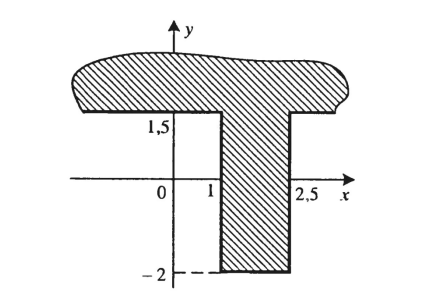
\includegraphics[width=0.5\textwidth]{2.png}
\end{center}

\item Згенерувати за допомогою модуля {\ttfamily random} випадкове дійсне число $x_0\in [-2; 2]$ і вивести на екран значення функції $y(x_0)$, якщо
$$
y(x)=\begin{cases}\ln (-2x), & \mbox{якщо } x<-0.5, \\
0, \mbox{якщо } -0.5\leqslant x\leqslant 1, \\
\sin(1-x), & \mbox{якщо } x>1.
\end{cases}
$$
Відповідь округлити до тисячних.
\end{enumerate}


\cleardoublepage

\LabHeader{2}{ 6}

\begin{enumerate}
\item Дано натуральне число. Чи правда, що воно закінчується на дві сімки?

\item Дано три довільні числа $x$, $y$, $z$. Обчислити та вивести на екран значення виразу
$$
F=\frac{5+\max\{x, y\}}{5-\min\{y, z\}},
$$
округляючи його до цілого.

\item Точка на площині задається своїми координатами $(x, y)$. Визначити, чи ця точка потрапляє в заштриховану частину площини.
\begin{center}
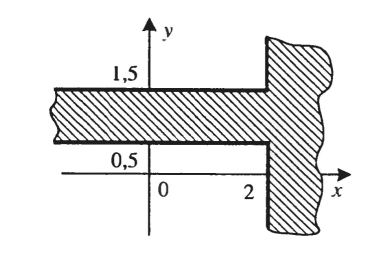
\includegraphics[width=0.5\textwidth]{1.png}
\end{center}

\item Згенерувати за допомогою модуля {\ttfamily random} випадкове дійсне число $x_0\in [-2; 2]$ і вивести на екран значення функції $y(x_0)$, якщо
$$
y(x)=\begin{cases}\cos x, & \mbox{якщо } x<0, \\
x^3+2x^2+1, & \mbox{якщо } 0\leqslant x<1.5, \\
0, & \mbox{якщо } x\geqslant 1.5.
\end{cases}
$$
Відповідь округлити до тисячних.

\end{enumerate}

\cleardoublepage

\LabHeader{2}{ 7}

\begin{enumerate}
\item Дане ціле число. Чи правда, що воно тризначне?

\item Дано три довільні числа $x$, $y$, $z$. Обчислити та вивести на екран значення виразу
$$
F=\frac{1+\max\{x+y, z\}}{\min\{y, z\}},
$$
округляючи його до цілого.

\item Точка на площині задається своїми координатами $(x, y)$. Визначити, чи ця точка потрапляє в заштриховану область $\mathcal{D}$.
\begin{center}
\begin{tikzpicture}
%graph
\draw[draw=Gainsboro,fill=Gainsboro] 
    plot[smooth,samples=100,domain=0:1] (\x,{0}) -- 
    plot[smooth,samples=100,domain=1:0] (\x,{1});
\draw[fill=Gainsboro] plot[smooth,samples=100,domain=1:2.71828] (\x,{ln(\x)}) -- 
    plot[smooth,samples=100,domain=2.71828:1] (\x,{1});
\draw[domain=0:4] plot (\x,{1});
\draw[samples=100,domain=.25:4,very thick] plot (\x,{ln(\x)}) node[above left]{$y=\ln x$};
%coordinate grid
\draw[->,>=Stealth] (-.5,0)--(4.5,0) node[above right]{$x$};
\draw[->,>=Stealth] (0,-1.5)--(0,2.5) node[above left]{$y$};
\foreach \x in {1,2,3,4}
    \draw (\x,2pt)--(\x,-2pt) node[below] {\footnotesize{$\x$}};
\foreach \y/\ytext in {1,2}
    \draw (2pt,\y)--(-2pt,\y) node[left] {\footnotesize{$\y$}};    
%labels 
\node at (.75,.5) {\large{$\mathcal{D}$}};
\end{tikzpicture}
\end{center}
%\begin{center}
%\includegraphics[scale=0.8]{14.png}
%\end{center}

\item Згенерувати за допомогою модуля {\ttfamily random} випадкове дійсне число $x_0\in [-2; 2]$ і вивести на екран значення функції $y(x_0)$, якщо
$$
y(x)=\begin{cases}\ln (-2x), & \mbox{якщо } x<-0.5, \\
0, \mbox{якщо } -0.5\leqslant x\leqslant 1, \\
\sin(1-x), & \mbox{якщо } x>1.
\end{cases}
$$
Відповідь округлити до тисячних.
\end{enumerate}

\cleardoublepage

\LabHeader{2}{ 8}

\begin{enumerate}
\item Дано тризначне натуральне число. Чи вірно, що воно є па\-лін\-дро\-мом\footnote[1]{\textbf{Паліндромом} називається число, яке дорівнює самому собі при прочитанні праворуч наліво. Наприклад, 121, 4554, 60606.}?

\item Дано три довільні числа $x$, $y$, $z$. Обчислити та вивести на екран значення виразу
$$
F=\frac{1+\max\{xyz, x+y+z\}}{1-\min\{x, y\}},
$$
округляючи його до цілого.

\item Крапка на площині задається своїми координатами $(x, y)$. Визначити, чи ця точка потрапляє в заштриховану частину площини.
\begin{center}
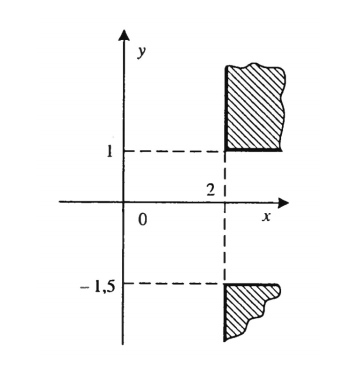
\includegraphics[width=0.5\textwidth]{3.png}
\end{center}

\clearpage

\item Згенерувати за допомогою модуля {\ttfamily random} випадкове дійсне число $x_0\in [-2; 2]$ і вивести на екран значення функції $y(x_0)$, якщо
$$
y(x)=\begin{cases}\cos x, & \mbox{якщо } x<0, \\
x^3+2x^2+1, & \mbox{якщо } 0\leqslant x<1.5, \\
0, & \mbox{якщо } x\geqslant 1.5.
\end{cases}
$$
Відповідь округлити до тисячних.
\end{enumerate}


\cleardoublepage

\LabHeader{2}{ 9}

\begin{enumerate}
\item Дано тризначне натуральне число. Чи правильно, що його цифри різні?

\item Дано три довільні числа $x$, $y$, $z$. Обчислити та вивести на екран значення виразу
$$
F=\frac{\max\{xy, z\}}{\min\{x+y, z\}-2},
$$
округляючи його до цілого.

\item Точка на площині задається своїми координатами $(x, y)$. Визначити, чи ця точка потрапляє в заштриховану область $\mathcal{D}$.
\begin{center}
\begin{tikzpicture}[scale=0.9]
%graph
\draw[draw=Gainsboro,fill=Gainsboro] 
    plot[smooth,samples=100,domain=-sqrt(2):sqrt(2)] (\x,{sqrt(4-\x*\x)}) -- 
    plot[smooth,samples=100,domain=0:sqrt(2)] (\x,\x) -- 
    plot[smooth,samples=100,domain=0:-sqrt(2)] (\x,-\x);
    \draw[draw=Gainsboro,fill=Gainsboro] 
    plot[smooth,samples=100,domain=-sqrt(2):sqrt(2)] (\x,{-sqrt(4-\x*\x)}) -- 
    plot[smooth,samples=100,domain=0:sqrt(2)] (\x,-\x) -- 
    plot[smooth,samples=100,domain=0:-sqrt(2)] (\x,\x);
\draw[draw=Gainsboro,fill=Gainsboro] plot[smooth,samples=100,domain=0:0] (\x,{sqrt(4-\x*\x)}) -- 
    plot[smooth,samples=100,domain=0:0] (\x,{0});
%\draw[domain=0:4] plot (\x,{1});
\draw[samples=100,domain=-sqrt(2):sqrt(2),very thick] plot (\x,{sqrt(4-\x*\x)});
\draw[samples=100,domain=-sqrt(2):sqrt(2),very thick] plot (\x,{-sqrt(4-\x*\x)});
\draw[very thick,domain=-sqrt(2):sqrt(2)] plot (\x,\x);
\draw[very thick,domain=-sqrt(2):sqrt(2)] plot (\x,-\x);
%\draw[very thick,fill=Gainsboro] 
%(-2,0)--(-1,0)--(-1,-1)--(1,-1)--(1,0)--(2,0);
%coordinate grid
\draw[->,>=Stealth] (-2.25,0)--(2.25,0) node[above right]{$x$};
\draw[->,>=Stealth] (0,-2.25)--(0,2.25) node[above left]{$y$};
\foreach \x in {-2,-1,1,2}
    \draw (\x,2pt)--(\x,-2pt) node[below] {\footnotesize{$\x$}};
\foreach \y/\ytext in {-2,-1,1,2}
    \draw (2pt,\y)--(-2pt,\y) node[left] {\footnotesize{$\y$}};    
%labels 
%\node at (.85,.85) {\large{$\mathcal{D}$}};
\node at (0.5,1.25) {\large{$\mathcal{D}$}};
\end{tikzpicture}
\end{center}
%\begin{center}
%\includegraphics[scale=0.5]{11.png}
%\end{center}

\item Згенерувати за допомогою модуля {\ttfamily random} випадкове дійсне число $x_0\in [-2; 2]$ і вивести на екран значення функції $y(x_0)$, якщо
$$
y(x)=\begin{cases}\ln (-2x), & \mbox{якщо } x<-0.5, \\
0, \mbox{якщо } -0.5\leqslant x\leqslant 1, \\
\sin(1-x), & \mbox{якщо } x>1.
\end{cases}
$$
Відповідь округлити до тисячних.
\end{enumerate}

\cleardoublepage

\LabHeader{2}{ 10}

\begin{enumerate}
\item Дано тризначне натуральне число. Чи правильно, що його цифри утворюють арифметичну прогресію?

\item Дано три довільні числа $x$, $y$, $z$. Обчислити та вивести на екран значення виразу
$$
F=\frac{5+\max\{x^2, y\}}{\max\{y, z\}},
$$
округляючи його до цілого.

\item Точка на площині задається своїми координатами $(x, y)$. Визначити, чи ця точка потрапляє в заштриховану область $\mathcal{D}$.
\begin{center}
\begin{tikzpicture}[scale=0.9]
%graph
\draw[draw=Gainsboro,fill=Gainsboro] 
    plot[smooth,samples=100,domain=-2:2] (\x,{sqrt(4-\x*\x)}) -- 
    plot[smooth,samples=100,domain=0:2] (\x,{0});
\draw[draw=Gainsboro,fill=Gainsboro] plot[smooth,samples=100,domain=0:0] (\x,{sqrt(4-\x*\x)}) -- 
    plot[smooth,samples=100,domain=0:0] (\x,{0});
%\draw[domain=0:4] plot (\x,{1});
\draw[samples=100,domain=-2:2,very thick] plot (\x,{sqrt(4-\x*\x)});
\draw[samples=100,domain=0:0,very thick] plot (\x,{sqrt(4-\x*\x)});
\draw[very thick,fill=Gainsboro] 
(-2,0)--(-1,0)--(-1,-1)--(1,-1)--(1,0)--(2,0);
%coordinate grid
\draw[->,>=Stealth] (-2.25,0)--(2.25,0) node[above right]{$x$};
\draw[->,>=Stealth] (0,-2.25)--(0,2.25) node[above left]{$y$};
\foreach \x in {-2,-1,1,2}
    \draw (\x,2pt)--(\x,-2pt) node[below] {\footnotesize{$\x$}};
\foreach \y/\ytext in {-2,-1,1,2}
    \draw (2pt,\y)--(-2pt,\y) node[left] {\footnotesize{$\y$}};    
%labels 
%\node at (.85,.85) {\large{$\mathcal{D}$}};
\node at (.85,.85) {\large{$\mathcal{D}$}};
\end{tikzpicture}
\end{center}
%\begin{center}
%\includegraphics[scale=0.5]{11.png}
%\end{center}

\item Згенерувати за допомогою модуля {\ttfamily random} випадкове дійсне число $x_0\in [-2; 2]$ і вивести на екран значення функції $y(x_0)$, якщо
$$
y(x)=\begin{cases}\cos x, & \mbox{якщо } x<0, \\
x^3+2x^2+1, & \mbox{якщо } 0\leqslant x<1.5, \\
0, & \mbox{якщо } x\geqslant 1.5.
\end{cases}
$$
Відповідь округлити до тисячних.
\end{enumerate}

\cleardoublepage

\LabHeader{2}{ 11}

\begin{enumerate}
\item Дано тризначне натуральне число. Чи правильно, що його цифри утворюють геометричну прогресію?

\item Дано три довільні числа $x$, $y$, $z$. Обчислити та вивести на екран значення виразу
$$
F=\frac{\max\{|x+y|, |z|\}}{\min\{y, z\}},
$$
округляючи його до цілого.

\item Точка на площині задається своїми координатами $(x, y)$. Визначити, чи ця точка потрапляє в заштриховану область $\mathcal{D}$.
\begin{center}
\begin{tikzpicture}[scale=0.9]
%graph
\draw[draw=Gainsboro,fill=Gainsboro] 
    plot[smooth,samples=100,domain=-2:2] (\x,{-sqrt(4-\x*\x)}) -- 
    plot[smooth,samples=100,domain=0:2] (\x,{0});
\draw[draw=Gainsboro,fill=Gainsboro] plot[smooth,samples=100,domain=0:0] (\x,{sqrt(4-\x*\x)}) -- 
    plot[smooth,samples=100,domain=0:0] (\x,{0});
%\draw[domain=0:4] plot (\x,{1});
\draw[samples=100,domain=-2:2,very thick] plot (\x,{-sqrt(4-\x*\x)});
\draw[samples=100,domain=0:0,very thick] plot (\x,{sqrt(4-\x*\x)});
\draw[very thick,fill=Gainsboro] 
(-2,0)--(-1,0)--(-1,1)--(1,1)--(1,0)--(2,0);
%coordinate grid
\draw[->,>=Stealth] (-2.25,0)--(2.25,0) node[above right]{$x$};
\draw[->,>=Stealth] (0,-2.25)--(0,2.25) node[above left]{$y$};
\foreach \x in {-2,-1,1,2}
    \draw (\x,2pt)--(\x,-2pt) node[below] {\footnotesize{$\x$}};
\foreach \y/\ytext in {-2,-1,1,2}
    \draw (2pt,\y)--(-2pt,\y) node[left] {\footnotesize{$\y$}};    
%labels 
%\node at (.85,.85) {\large{$\mathcal{D}$}};
\node at (.85,-.85) {\large{$\mathcal{D}$}};
\end{tikzpicture}
\end{center}
%\begin{center}
%\includegraphics[scale=0.5]{11.png}
%\end{center}

\item Згенерувати за допомогою модуля {\ttfamily random} випадкове дійсне число $x_0\in [-2; 2]$ і вивести на екран значення функції $y(x_0)$, якщо
$$
y(x)=\begin{cases}\cos x, & \mbox{якщо } x<0, \\
x^3+2x^2+1, & \mbox{якщо } 0\leqslant x<1.5, \\
0, & \mbox{якщо } x\geqslant 1.5.
\end{cases}
$$
Відповідь округлити до тисячних.
\end{enumerate}

\cleardoublepage

\LabHeader{2}{ 12}

\begin{enumerate}
\item Дано двозначне натуральне число. Чи вірно, що сума його цифр кратна п'яти?

\item Дано три довільні числа $x$, $y$, $z$. Обчислити та вивести на екран значення виразу
$$
F=\frac{\max\{x+y+z, z\}}{3-\min\{x, yz\}},
$$
округляючи його до цілого.

\item Точка на площині задається своїми координатами $(x, y)$. Визначити, чи ця точка потрапляє в заштриховану область $\mathcal{D}$.
\begin{center}
\begin{tikzpicture}[scale=0.9]
%graph
\draw[draw=Gainsboro,fill=Gainsboro] 
    plot[smooth,samples=100,domain=-2:0] (\x,{sqrt(4-\x*\x)}) -- 
    plot[smooth,samples=100,domain=0:-1] (\x,{sqrt(1-\x*\x)});
\draw[draw=Gainsboro,fill=Gainsboro] 
    plot[smooth,samples=100,domain=0:2] (\x,{-sqrt(4-\x*\x)}) -- 
    plot[smooth,samples=100,domain=1:0] (\x,{-sqrt(1-\x*\x)});
%\draw[domain=0:4] plot (\x,{1});
\draw[samples=100,domain=-2:0,very thick] plot (\x,{sqrt(4-\x*\x)});
\draw[samples=100,domain=0:2,very thick] plot (\x,{-sqrt(4-\x*\x)});
\draw[samples=100,domain=-1:0,very thick] plot (\x,{sqrt(1-\x*\x)});
\draw[samples=100,domain=0:1,very thick] plot (\x,{-sqrt(1-\x*\x)});
%coordinate grid
\draw[->,>=Stealth] (-2.5,0)--(2.5,0) node[above right]{$x$};
\draw[->,>=Stealth] (0,-2.5)--(0,2.5) node[above left]{$y$};
\foreach \x in {-2,-1,1,2}
    \draw (\x,0) node[below right] {\footnotesize{$\x$}};
\foreach \y/\ytext in {-2,-1,1,2}
    \draw (0,\y) node[above left] {\footnotesize{$\y$}};    
%labels 
\node at (-1,1) {\large{$\mathcal{D}$}};
\node at (1,-1) {\large{$\mathcal{D}$}};
\end{tikzpicture}
\end{center}
%\begin{center}
%\includegraphics[scale=0.5]{12.png}
%\end{center}

\item Згенерувати за допомогою модуля {\ttfamily random} випадкове дійсне число $x_0\in [-2; 2]$ і вивести на екран значення функції $y(x_0)$, якщо
$$
y(x)=\begin{cases}\cos x, & \mbox{якщо } x<0, \\
x^3+2x^2+1, & \mbox{якщо } 0\leqslant x<1.5, \\
0, & \mbox{якщо } x\geqslant 1.5.
\end{cases}
$$
Відповідь округлити до тисячних.
\end{enumerate}

\cleardoublepage

\LabHeader{2}{ 13}

\begin{enumerate}
\item Дано тризначне натуральне число. Чи вірно, що воно складається лише з парних цифр (0 вважати парною цифрою)?

\item Дано три довільні числа $x$, $y$, $z$. Обчислити та вивести на екран значення виразу
$$
F=\frac{1+\max\{x, z\}}{1-\min\{xy, z^2\}},
$$
округляючи його до цілого.

\item Точка на площині задається своїми координатами $(x, y)$. Визначити, чи ця точка потрапляє в заштриховану область $\mathcal{D}$.
\begin{center}
\begin{tikzpicture}[scale=0.9]
%graph
\draw[draw=Gainsboro,fill=Gainsboro] 
    plot[smooth,samples=100,domain=-2:0] (\x,{-sqrt(4-\x*\x)}) -- 
    plot[smooth,samples=100,domain=0:-1] (\x,{-sqrt(1-\x*\x)});
\draw[draw=Gainsboro,fill=Gainsboro] 
    plot[smooth,samples=100,domain=0:2] (\x,{sqrt(4-\x*\x)}) -- 
    plot[smooth,samples=100,domain=1:0] (\x,{sqrt(1-\x*\x)});
%\draw[domain=0:4] plot (\x,{1});
\draw[samples=100,domain=-2:0,very thick] plot (\x,{-sqrt(4-\x*\x)});
\draw[samples=100,domain=0:2,very thick] plot (\x,{sqrt(4-\x*\x)});
\draw[samples=100,domain=-1:0,very thick] plot (\x,{-sqrt(1-\x*\x)});
\draw[samples=100,domain=0:1,very thick] plot (\x,{sqrt(1-\x*\x)});
%coordinate grid
\draw[->,>=Stealth] (-2.5,0)--(2.5,0) node[above right]{$x$};
\draw[->,>=Stealth] (0,-2.5)--(0,2.5) node[above left]{$y$};
\foreach \x in {-2,-1,1,2}
    \draw (\x,0) node[below right] {\footnotesize{$\x$}};
\foreach \y/\ytext in {-2,-1,1,2}
    \draw (0,\y) node[above left] {\footnotesize{$\y$}};    
%labels 
\node at (1,1) {\large{$\mathcal{D}$}};
\node at (-1,-1) {\large{$\mathcal{D}$}};
\end{tikzpicture}
\end{center}
%\begin{center}
%\includegraphics[scale=0.5]{12.png}
%\end{center}

\item Згенерувати за допомогою модуля {\ttfamily random} випадкове дійсне число $x_0\in [-2; 2]$ і вивести на екран значення функції $y(x_0)$, якщо
$$
y(x)=\begin{cases}\ln (-2x), & \mbox{якщо } x<-0.5, \\
0, \mbox{якщо } -0.5\leqslant x\leqslant 1, \\
\sin(1-x), & \mbox{якщо } x>1.
\end{cases}
$$
Відповідь округлити до тисячних.
\end{enumerate}

\cleardoublepage

\LabHeader{2}{ 14}

\begin{enumerate}
\item Дано натуральне число. Чи правда, що воно закінчується двома нулями?

\item Дано три довільні числа $x$, $y$, $z$. Обчислити та вивести на екран значення виразу
$$
F=\frac{\max\{x+y, y+z\}}{\min\{xy, yz\}},
$$
округляючи його до цілого.

\item Точка на площині задається своїми координатами $(x, y)$. Визначити, чи ця точка потрапляє в заштриховану частину площини.
\begin{center}
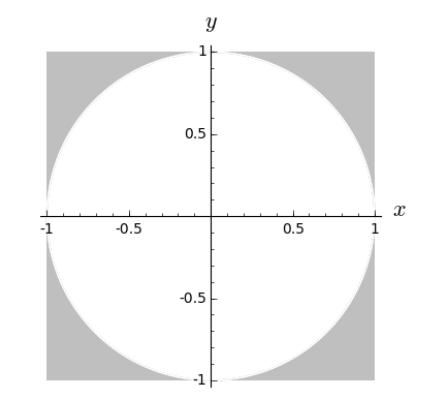
\includegraphics[width=0.7\textwidth]{9.png}
\end{center}

\clearpage

\item Згенерувати за допомогою модуля {\ttfamily random} випадкове дійсне число $x_0\in [-2; 2]$ і вивести на екран значення функції $y(x_0)$, якщо
$$
y(x)=\begin{cases}\cos x, & \mbox{якщо } x<0, \\
x^3+2x^2+1, & \mbox{якщо } 0\leqslant x<1.5, \\
0, & \mbox{якщо } x\geqslant 1.5.
\end{cases}
$$
Відповідь округлити до тисячних.

\end{enumerate}

\cleardoublepage

\LabHeader{2}{ 15}

\begin{enumerate}
\item Дано тризначне натуральне число. Чи вірно, що його цифри рас-по-ло-же-ни в порядку убування?

\item Дано три довільні числа $x$, $y$, $z$. Обчислити та вивести на екран значення виразу
$$
F=\frac{\max\{x, z\}-1}{\min\{x+y, y+z\}},
$$
округляючи його до цілого.

\item Точка на площині задається своїми координатами $(x, y)$. Визначити, чи ця точка потрапляє в заштриховану частину площини.
\begin{center}
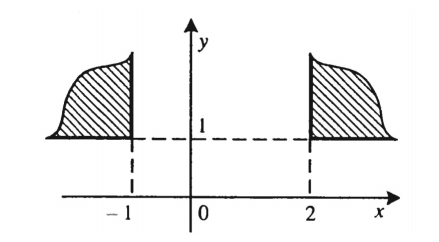
\includegraphics[width=0.7\textwidth]{10.png}
\end{center}

\item Згенерувати за допомогою модуля {\ttfamily random} випадкове дійсне число $x_0\in [-2; 2]$ і вивести на екран значення функції $y(x_0)$, якщо
$$
y(x)=\begin{cases}\ln (-2x), & \mbox{якщо } x<-0.5, \\
0, \mbox{якщо } -0.5\leqslant x\leqslant 1, \\
\sin(1-x), & \mbox{якщо } x>1.
\end{cases}
$$
Відповідь округлити до тисячних.
\end{enumerate}

\cleardoublepage

\LabHeader{2}{ 16}

\begin{enumerate}
\item Дано тризначне натуральне число. Чи вірно, що його друга цифра точно дорівнює сумі першої і третьої?

\item Дано три довільні числа $x$, $y$, $z$. Обчислити та вивести на екран значення виразу
$$
F=\frac{\max\{x, y\}}{1-\min\{xy, yz\}},
$$
округляючи його до цілого.

\item Крапка на площині задається своїми координатами $(x, y)$. Визначити, чи ця точка потрапляє в заштриховану область $\mathcal{D}$.
\begin{center}
\begin{tikzpicture}[scale=0.9]
%graph
\draw[draw=Gainsboro,fill=Gainsboro] 
    plot[smooth,samples=100,domain=-2:0] (\x,{-sqrt(4-\x*\x)}) -- 
    plot[smooth,samples=100,domain=0:2] (\x,{0});
\draw[draw=Gainsboro,fill=Gainsboro] plot[smooth,samples=100,domain=0:2] (\x,{sqrt(4-\x*\x)}) -- 
    plot[smooth,samples=100,domain=-2:0] (\x,{0});
%\draw[domain=0:4] plot (\x,{1});
\draw[samples=100,domain=-2:0,very thick] plot (\x,{-sqrt(4-\x*\x)});
\draw[samples=100,domain=0:2,very thick] plot (\x,{sqrt(4-\x*\x)});
%coordinate grid
\draw[->,>=Stealth] (-2.25,0)--(2.25,0) node[above right]{$x$};
\draw[->,>=Stealth] (0,-2.25)--(0,2.25) node[above left]{$y$};
\foreach \x in {-2,-1,1,2}
    \draw (\x,2pt)--(\x,-2pt) node[below] {\footnotesize{$\x$}};
\foreach \y/\ytext in {-2,-1,1,2}
    \draw (2pt,\y)--(-2pt,\y) node[left] {\footnotesize{$\y$}};    
%labels 
\node at (.85,.85) {\large{$\mathcal{D}$}};
\node at (-.85,-.85) {\large{$\mathcal{D}$}};
\end{tikzpicture}
\end{center}
%\begin{center}
%\includegraphics[scale=0.5]{11.png}
%\end{center}

\item Згенерувати за допомогою модуля {\ttfamily random} випадкове дійсне число $x_0\in [-2; 2]$ і вивести на екран значення функції $y(x_0)$, якщо
$$
y(x)=\begin{cases}\cos x, & \mbox{якщо } x<0, \\
x^3+2x^2+1, & \mbox{якщо } 0\leqslant x<1.5, \\
0, & \mbox{якщо } x\geqslant 1.5.
\end{cases}
$$
Відповідь округлити до тисячних.
\end{enumerate}

\cleardoublepage

\LabHeader{2}{ 17}

\begin{enumerate}
\item Дано двозначне натуральне число. Чи вірно, що сума його цифр кратна п'яти?

\item Дано три довільні числа $x$, $y$, $z$. Обчислити та вивести на екран значення виразу
$$
F=\frac{\max\{x+y+z, z\}}{3-\min\{x, yz\}},
$$
округляючи його до цілого.

\item Точка на площині задається своїми координатами $(x, y)$. Визначити, чи ця точка потрапляє в заштриховану область $\mathcal{D}$.
\begin{center}
\begin{tikzpicture}[scale=0.9]
%graph
\draw[draw=Gainsboro,fill=Gainsboro] 
    plot[smooth,samples=100,domain=-2:0] (\x,{sqrt(4-\x*\x)}) -- 
    plot[smooth,samples=100,domain=0:-1] (\x,{sqrt(1-\x*\x)});
\draw[draw=Gainsboro,fill=Gainsboro] 
    plot[smooth,samples=100,domain=0:2] (\x,{-sqrt(4-\x*\x)}) -- 
    plot[smooth,samples=100,domain=1:0] (\x,{-sqrt(1-\x*\x)});
%\draw[domain=0:4] plot (\x,{1});
\draw[samples=100,domain=-2:0,very thick] plot (\x,{sqrt(4-\x*\x)});
\draw[samples=100,domain=0:2,very thick] plot (\x,{-sqrt(4-\x*\x)});
\draw[samples=100,domain=-1:0,very thick] plot (\x,{sqrt(1-\x*\x)});
\draw[samples=100,domain=0:1,very thick] plot (\x,{-sqrt(1-\x*\x)});
%coordinate grid
\draw[->,>=Stealth] (-2.5,0)--(2.5,0) node[above right]{$x$};
\draw[->,>=Stealth] (0,-2.5)--(0,2.5) node[above left]{$y$};
\foreach \x in {-2,-1,1,2}
    \draw (\x,0) node[below right] {\footnotesize{$\x$}};
\foreach \y/\ytext in {-2,-1,1,2}
    \draw (0,\y) node[above left] {\footnotesize{$\y$}};    
%labels 
\node at (-1,1) {\large{$\mathcal{D}$}};
\node at (1,-1) {\large{$\mathcal{D}$}};
\end{tikzpicture}
\end{center}
%\begin{center}
%\includegraphics[scale=0.5]{12.png}
%\end{center}

\item Згенерувати за допомогою модуля {\ttfamily random} випадкове дійсне число $x_0\in [-2; 2]$ і вивести на екран значення функції $y(x_0)$, якщо
$$
y(x)=\begin{cases}\cos x, & \mbox{якщо } x<0, \\
x^3+2x^2+1, & \mbox{якщо } 0\leqslant x<1.5, \\
0, & \mbox{якщо } x\geqslant 1.5.
\end{cases}
$$
Відповідь округлити до тисячних.
\end{enumerate}

\cleardoublepage

\LabHeader{2}{ 18}

\begin{enumerate}
\item Дано тризначне натуральне число. Чи вірно, що його цифри рас-по-ло-же-ни в порядку убування?

\item Дано три довільні числа $x$, $y$, $z$. Обчислити та вивести на екран значення виразу
$$
F=\frac{\max\{x, z\}-1}{\min\{x+y, y+z\}},
$$
округляючи його до цілого.

\item Точка на площині задається своїми координатами $(x, y)$. Визначити, чи ця точка потрапляє в заштриховану частину площини.
\begin{center}
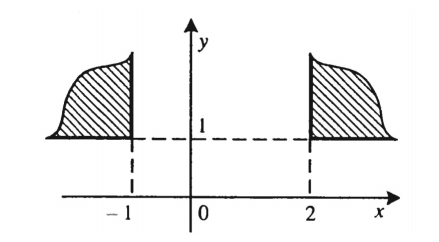
\includegraphics[width=0.7\textwidth]{10.png}
\end{center}

\item Згенерувати за допомогою модуля {\ttfamily random} випадкове дійсне число $x_0\in [-2; 2]$ і вивести на екран значення функції $y(x_0)$, якщо
$$
y(x)=\begin{cases}\ln (-2x), & \mbox{якщо } x<-0.5, \\
0, \mbox{якщо } -0.5\leqslant x\leqslant 1, \\
\sin(1-x), & \mbox{якщо } x>1.
\end{cases}
$$
Відповідь округлити до тисячних.
\end{enumerate}
